% ============================================================
%  يُترجَم بـ XeLaTeX  (في Overleaf: Menu → Compiler → XeLaTeX)
%  الخط: Amiri (متوفر في Overleaf، أو حمّله من github.com/aliftype/amiri)
% ============================================================
\documentclass[12pt,a4paper]{article}
\usepackage[a4paper,margin=1.7cm,top=2.3cm,bottom=2.9cm,headheight=15pt,footskip=1.5cm]{geometry}
\usepackage{amsmath,amssymb}
\usepackage{icomma}
\usepackage[english,bidi=default,layout=lists]{babel}
\babelprovide[import,main]{arabic}
\babelfont{rm}[Scale=1.08]{Amiri}
\babelfont{sf}[Scale=1.08]{Amiri}
\usepackage[most]{tcolorbox}
\usepackage{tikz}
\usetikzlibrary{arrows.meta,calc,shadings}
\usepackage{array}
\usepackage{colortbl}
\usepackage{fancyhdr}
\usepackage{titlesec}
\usepackage{enumitem}
\usepackage{collcell}
\usepackage{needspace}
\usepackage{etoolbox}
% أعمدة جداول تُكتب خلاياها بالعربية في الاتجاه الصحيح
\newcolumntype{C}{>{\collectcell\ar}c<{\endcollectcell}}
% تجنب عنوان يتيم في أسفل الصفحة
\pretocmd{\section}{\Needspace{15\baselineskip}}{}{}
\pretocmd{\subsection}{\Needspace{11\baselineskip}}{}{}

% ---------- الألوان ----------
\definecolor{cDef}{HTML}{1F4E9C}
\definecolor{cThm}{HTML}{B3261E}
\definecolor{cRem}{HTML}{2E7D32}
\definecolor{cEx}{HTML}{C76B00}
\definecolor{cMeth}{HTML}{6A1B9A}
\definecolor{cSol}{HTML}{00695C}
\definecolor{cSec}{HTML}{1F3A68}

% ---------- العناوين ----------
\titleformat{\section}{\Large\bfseries\color{cSec}}{\thesection.}{0.6em}{}[{\color{cSec!60}\titlerule[1pt]}]
\titleformat{\subsection}{\large\bfseries\color{cThm!85!black}}{\thesubsection.}{0.5em}{}
\titlespacing*{\section}{0pt}{14pt}{8pt}
\titlespacing*{\subsection}{0pt}{10pt}{5pt}
\setlength{\parindent}{0pt}
\setlength{\parskip}{4pt}
\setlist{itemsep=2pt,topsep=3pt}

% ---------- الصناديق (تُرسم في سياق LTR ويُكتب محتواها بالعربية) ----------
\newtcolorbox{arbox}[3][]{enhanced,
  colback=#2!5,colframe=#2!80!black,arc=2mm,boxrule=0.8pt,
  left=6pt,right=6pt,top=8pt,bottom=5pt,
  fonttitle=\bfseries,coltitle=white,
  title={\foreignlanguage{arabic}{#3}},
  attach boxed title to top right={xshift=-5mm,yshift=-3mm},
  boxed title style={colback=#2!80!black,arc=1.5mm,boxrule=0pt},
  before upper={\selectlanguage{arabic}},
  before skip=8pt,after skip=8pt,breakable,#1}
\newenvironment{BOX}[2]{\begin{otherlanguage}{english}\begin{arbox}{#1}{#2}}{\end{arbox}\end{otherlanguage}}
\newenvironment{tarif}[1][تعريف]{\begin{BOX}{cDef}{#1}}{\end{BOX}}
\newenvironment{khassia}[1][خاصية]{\begin{BOX}{cThm}{#1}}{\end{BOX}}
\newenvironment{molahada}[1][ملاحظة]{\begin{BOX}{cRem}{#1}}{\end{BOX}}
\newenvironment{mithal}[1][مثال]{\begin{BOX}{cEx}{#1}}{\end{BOX}}
\newenvironment{tariqa}[1][طريقة]{\begin{BOX}{cMeth}{#1}}{\end{BOX}}

% ---------- التمارين والحلول ----------
\newcounter{exo}
\newenvironment{tamrin}[1]{\stepcounter{exo}\begin{BOX}{cSec}{التمرين \theexo: #1}}{\end{BOX}}
\newenvironment{hal}{\Needspace{12\baselineskip}\begin{otherlanguage}{english}\begin{arbox}[breakable]{cSol}{حل التمرين \theexo}}{\end{arbox}\end{otherlanguage}}

% رسومات TikZ تُوضع في سياق LTR
\newenvironment{LTR}{\begin{otherlanguage}{english}}{\end{otherlanguage}}
\newcommand{\ar}[1]{\foreignlanguage{arabic}{#1}}

% ---------- رموز ----------
% نقاط الحذف داخل الرياضيات (\dots يسبب خللاً في الاتجاه مع babel)
\renewcommand{\dots}{\mathinner{\ldotp\ldotp\ldotp}}
\renewcommand{\ldots}{\mathinner{\ldotp\ldotp\ldotp}}
\renewcommand{\cdots}{\mathinner{\cdotp\cdotp\cdotp}}
\newcommand{\N}{\mathbb{N}}
\newcommand{\Z}{\mathbb{Z}}
\newcommand{\D}{\mathbb{D}}
\newcommand{\Q}{\mathbb{Q}}
\newcommand{\R}{\mathbb{R}}
\newcommand{\pgcd}{\operatorname{PGCD}}
\newcommand{\ppcm}{\operatorname{PPCM}}

% ---------- تمثيل مجال على مستقيم عددي ----------
% \NLseg{a}{b}{[}{]}  مجال محدود
\newcommand{\NLseg}[4]{\begin{LTR}\begin{tikzpicture}[baseline=-0.6ex]
 \draw[-{Stealth[length=2mm]},gray!70](0,0)--(3.4,0);
 \draw[line width=2pt,cThm!80!black](0.7,0)--(2.7,0);
 \node[cThm!80!black,font=\LARGE] at (0.7,0){$#3$};
 \node[cThm!80!black,font=\LARGE] at (2.7,0){$#4$};
 \node[below=3pt,font=\footnotesize] at (0.7,0){$#1$};
 \node[below=3pt,font=\footnotesize] at (2.7,0){$#2$};
\end{tikzpicture}\end{LTR}}
% \NLright{a}{[}  مجال نحو +∞
\newcommand{\NLright}[2]{\begin{LTR}\begin{tikzpicture}[baseline=-0.6ex]
 \draw[-{Stealth[length=2mm]},gray!70](0,0)--(3.4,0);
 \draw[line width=2pt,cThm!80!black](1.3,0)--(3.3,0);
 \node[cThm!80!black,font=\LARGE] at (1.3,0){$#2$};
 \node[below=3pt,font=\footnotesize] at (1.3,0){$#1$};
\end{tikzpicture}\end{LTR}}
% \NLleft{b}{]}  مجال نحو −∞
\newcommand{\NLleft}[2]{\begin{LTR}\begin{tikzpicture}[baseline=-0.6ex]
 \draw[-{Stealth[length=2mm]},gray!70](0,0)--(3.4,0);
 \draw[line width=2pt,cThm!80!black](0.05,0)--(2.1,0);
 \node[cThm!80!black,font=\LARGE] at (2.1,0){$#2$};
 \node[below=3pt,font=\footnotesize] at (2.1,0){$#1$};
\end{tikzpicture}\end{LTR}}

% ---------- أيقونات مواقع التواصل (مرسومة بـ TikZ، لا تحتاج أي حزمة) ----------
\definecolor{cFB}{HTML}{1877F2}
\definecolor{cTG}{HTML}{229ED9}
\definecolor{cIG1}{HTML}{FEDA75}
\definecolor{cIG2}{HTML}{D62976}
\definecolor{cIG3}{HTML}{4F5BD5}
\newcommand{\fbicon}{\begin{LTR}\begin{tikzpicture}[baseline=-0.75ex,x=1em,y=1em]
 \fill[cFB] (0,0) circle (0.55);
 \node[white,inner sep=0,font=\usefont{TU}{lmss}{bx}{n}\small] at (0.04,-0.02) {f};
\end{tikzpicture}\end{LTR}}
\newcommand{\igicon}{\begin{LTR}
\begin{tikzpicture}[baseline=-0.75ex,x=1em,y=1em]
 \shade[lower left=cIG1,lower right=cIG2,upper left=cIG2,upper right=cIG3,rounded corners=0.28em] (-0.55,-0.55) rectangle (0.55,0.55);
 \draw[white,line width=0.09em,rounded corners=0.18em] (-0.36,-0.36) rectangle (0.36,0.36);
 \draw[white,line width=0.09em] (0,0) circle (0.17);
 \fill[white] (0.22,0.22) circle (0.05);
\end{tikzpicture}\end{LTR}}
\newcommand{\tgicon}{\begin{LTR}
\begin{tikzpicture}[baseline=-0.75ex,x=1em,y=1em]
 \fill[cTG] (0,0) circle (0.55);
 \fill[white] (-0.33,0.0) -- (0.32,0.27) -- (0.2,-0.3) -- (0.0,-0.15) -- (-0.08,-0.28) -- (-0.08,-0.08) -- cycle;
 \fill[cTG!70!black] (-0.08,-0.08) -- (0.25,0.2) -- (0.0,-0.15) -- (-0.08,-0.28) -- cycle;
\end{tikzpicture}\end{LTR}}
% سطر مواقع التواصل أسفل كل صفحة
% (يُكتب السطر بترتيب بصري من اليسار إلى اليمين: الأيقونة يمين كل اسم)
\newcommand{\PageBox}{\begin{LTR}\tikz[baseline=(p.base)]\node[fill=black,text=white,inner sep=2.5pt,minimum width=1.6em,minimum height=1.3em,font=\usefont{TU}{lmss}{bx}{n}\small](p){\ifnum\value{page}<10 0\fi\arabic{page}};\end{LTR}}
\newcommand{\SocialRow}{\begin{otherlanguage}{english}%
 \ar{\textbf{الأستاذ سوايسية هشام للرياضيات}}\ \tgicon\hfill
 \textbf{prof\_hicham\_math}\ \igicon\hfill
 \ar{\textbf{الأستاذ سوايسية هشام للرياضيات}}\ \fbicon\hspace{2.2em}\PageBox\end{otherlanguage}}
% ---------- رأس وتذييل الصفحة ----------
\pagestyle{fancy}
\fancyhf{}
\renewcommand{\headrulewidth}{0.6pt}
\renewcommand{\footrulewidth}{0.4pt}
% \SetHeader{يمين الرأس}{يسار الرأس}{يمين التذييل}{يسار التذييل}
\newcommand{\SetHeader}[2]{%
 \fancyhead[C]{\parbox{\textwidth}{\ar{#1\hfill #2}}}%
 \fancyfoot[C]{\parbox{\textwidth}{\small\SocialRow}}}

\usepackage{tkz-tab}
\usepackage{multicol}
% جدول تغيرات / إشارة (يُرسم في سياق LTR)
\newenvironment{TAB}{\par\begin{center}\begin{LTR}\begin{tikzpicture}[scale=0.95,every node/.style={font=\small}]}{\end{tikzpicture}\end{LTR}\end{center}}
% معلم بشبكة: \begin{GR}{xmin}{xmax}{ymin}{ymax}{unit cm}
\newenvironment{GR}[5]{\par\begin{center}\begin{LTR}\begin{tikzpicture}[x=#5cm,y=#5cm,font=\footnotesize]
 \def\xmn{#1}\def\xmx{#2}\def\ymn{#3}\def\ymx{#4}
 \draw[gray!25,very thin] (#1,#3) grid (#2,#4);
 \draw[-{Stealth[length=2mm]}] (#1,0)--(#2+0.3,0) node[below left]{$x$};
 \draw[-{Stealth[length=2mm]}] (0,#3)--(0,#4+0.3) node[below left]{$y$};
 \node[below left] at (0,0){$O$};
 \draw[very thick,-{Stealth[length=1.6mm]}] (0,0)--(1,0) node[below,pos=.55]{$\vec i$};
 \draw[very thick,-{Stealth[length=1.6mm]}] (0,0)--(0,1) node[left,pos=.55]{$\vec j$};
 \begin{scope}\clip (#1,#3) rectangle (#2,#4);}
{\end{scope}\end{tikzpicture}\end{LTR}\end{center}}
\newcommand{\Ticks}[2]{\foreach \t in {#1} \node[below,font=\scriptsize] at (\t,0){$\t$}; \foreach \t in {#2} \node[left,font=\scriptsize] at (0,\t){$\t$};}
\newcommand{\bx}[1]{\ensuremath{\colorbox{cDef!12}{$\displaystyle #1$}}}
\newcommand{\hl}[1]{\ensuremath{\colorbox{cEx!20}{$\displaystyle #1$}}}
\newcommand{\Lim}[1]{\displaystyle\lim_{x\to #1}}
\newcommand{\Cf}{(C_f)}
\newenvironment{qst}{\begin{enumerate}[label=\protect\circled{\arabic*},leftmargin=*]}{\end{enumerate}}
\newcommand{\circled}[1]{\foreignlanguage{english}{\tikz[baseline=(c.base)]\node[circle,fill=cDef,text=white,inner sep=1.2pt,font=\scriptsize\bfseries](c){#1};}}
% عمودان: \TwoCol{عرض اليسار}{محتوى اليسار}{عرض اليمين}{محتوى اليمين}  (آمن مع TikZ)
\newcommand{\TwoCol}[4]{\par\begin{LTR}\noindent\begin{minipage}[t]{#1\textwidth}\selectlanguage{arabic}#2\end{minipage}\hfill\begin{minipage}[t]{#3\textwidth}\selectlanguage{arabic}#4\end{minipage}\end{LTR}\par}
\newcommand{\un}{(u_n)}\newcommand{\vn}{(v_n)}
% برهان بالتراجع: \Rec{الخاصية P(n)}{التحقق من P(0)}{البرهان على الوراثة}
\newcommand{\Rec}[3]{\textbf{برهان بالتراجع:} نسمي $P(n)$ الخاصية: «#1».
\begin{itemize}
\item \textbf{التحقق:} #2
\item \textbf{الوراثة:} نفرض أن $P(n)$ صحيحة ونبرهن صحة $P(n+1)$: #3
\item \textbf{الخلاصة:} حسب مبدأ الاستدلال بالتراجع، $P(n)$ صحيحة من أجل كل عدد طبيعي $n$.
\end{itemize}}
\newcommand{\src}[1]{{\footnotesize\textbf{#1}}\par}
\newcommand{\ok}{$\textcolor{cRem}{\checkmark}$}
\newcommand{\limn}{\displaystyle\lim_{n\to+\infty}}
% أسئلة فرعية (أ) (ب) (جـ) كل سؤال في سطر
\newenvironment{sq}{\begin{itemize}[leftmargin=2.4em,itemsep=3pt]}{\end{itemize}}
\newcommand{\qa}{\item[(أ)]}\newcommand{\qb}{\item[(ب)]}\newcommand{\qc}{\item[(جـ)]}\newcommand{\qd}{\item[(د)]}\newcommand{\qe}{\item[(هـ)]}
\newcommand{\pa}{\par\smallskip\textbf{(أ)} }\newcommand{\pb}{\par\smallskip\textbf{(ب)} }\newcommand{\pc}{\par\smallskip\textbf{(جـ)} }\newcommand{\pd}{\par\smallskip\textbf{(د)} }\newcommand{\pe}{\par\smallskip\textbf{(هـ)} }
\newcommand{\ccl}[1]{\par\textbf{الخلاصة:} #1}

\SetHeader{\small\bfseries\color{cSec}ملخص: الاحتمالات}{\small\color{cSec}السنة الثانية ثانوي -- الشعب العلمية}
\begin{document}
\newcolumntype{M}[1]{>{\centering\arraybackslash}p{#1}}
\newcommand{\RL}[4]{\TwoCol{#3}{#4}{#1}{#2}}
\newenvironment{tmr}{\stepcounter{exo}\begin{BOX}{cSec}{تمرين محلول \theexo}}{\end{BOX}}
\newcommand{\card}{\operatorname{Card}}
\begin{LTR}
\begin{tcolorbox}[enhanced,colback=cSec,colframe=cSec,arc=3mm,halign=center,boxrule=0pt,top=12pt,bottom=12pt,before upper={\selectlanguage{arabic}}]
{\color{white}\fontsize{28}{34}\selectfont\bfseries الاحتمالات}\\[8pt]
{\color{white}\large ملخص شامل مع أمثلة وتمارين محلولة خطوة بخطوة}\\[5pt]
{\color{white}\large السنة الثانية ثانوي -- الشعب العلمية (رياضيات ، تقني رياضي ، علوم تجريبية)}
\end{tcolorbox}
\end{LTR}

\begin{BOX}{cSec}{محتوى الملخص (حسب ترتيب التوزيع السنوي)}
\begin{center}
\begin{tabular}{p{0.44\textwidth}p{0.44\textwidth}}
6. أدوات العدّ: الجداول المزدوجة وشجرة الإمكانيات & 1. التجربة العشوائية ، التواترات والمحاكاة\\
7. خواص الاحتمال & 2. مصطلحات الاحتمالات (لغة الحوادث)\\
8. المتغير العشوائي وقانون احتماله & 3. قانون الاحتمال على مجموعة منتهية\\
9. الأمل والتباين والانحراف المعياري لمتغير عشوائي & 4. الأمل والتباين والانحراف المعياري لقانون احتمال\\
10. خلاصة الطرائق & 5. تساوي الاحتمال
\end{tabular}
\end{center}
\end{BOX}

% =====================================================================
\section{التجربة العشوائية ، التواترات والمحاكاة}
\begin{tarif}[التجربة العشوائية]
\textbf{التجربة العشوائية} هي كل تجربة نعرف مسبقاً جميع نتائجها الممكنة ، لكن لا يمكن توقّع النتيجة التي ستظهر قبل إجرائها.\par
كل نتيجة ممكنة تسمى \textbf{مخرجاً} (أو إمكانية) ، ومجموعة كل المخارج تسمى \textbf{مجموعة الإمكانيات} ونرمز لها بالرمز $\Omega$.
\end{tarif}
\begin{mithal}
\begin{itemize}
\item رمي قطعة نقدية: \ $\Omega=\{F;P\}$ \ ($F$: الوجه ، $P$: الظهر).
\item رمي زهرة نرد مرقمة من $1$ إلى $6$: \ $\Omega=\{1;2;3;4;5;6\}$.
\item سحب كرية من كيس به كريات مرقمة من $1$ إلى $5$: \ $\Omega=\{1;2;3;4;5\}$.
\end{itemize}
\end{mithal}

\begin{tarif}[التواتر]
نكرر تجربة عشوائية $N$ مرة ، ونسجل عدد مرات ظهور كل مخرج $x_i$ ، وهو التكرار $n_i$.\par
\textbf{تواتر} المخرج $x_i$ هو العدد: \ \bx{f_i=\dfrac{n_i}{N}} \ ، \ ولدينا دائماً: \ $0\le f_i\le1$ \ و \ $f_1+f_2+\dots+f_k=1$.
\end{tarif}

\begin{khassia}[استقرار التواترات]
عندما يكبر عدد التكرارات $N$ (مقاس العينة) ، تقل تذبذبات التواترات $f_i$ وتقترب من قيم نظرية ثابتة $p_i$ نسميها \textbf{احتمالات} المخارج.\par
نميز بين \textbf{التواتر التجريبي} $f_i$ (يتغير من عينة إلى أخرى) و\textbf{التواتر النظري} $p_i$ (ثابت).
\end{khassia}

\begin{mithal}[رمي قطعة نقدية]
\begin{center}
\renewcommand{\arraystretch}{1.3}
\begin{tabular}{|C|c|c|c|c|}\hline
\rowcolor{cSec!12}عدد الرميات $N$ & $10$ & $100$ & $1000$ & $10000$\\
\hline
تواتر الوجه $F$ & $0{,}7$ & $0{,}56$ & $0{,}521$ & $0{,}499$\\
\hline
\end{tabular}
\end{center}
كلما كبر $N$ اقترب تواتر ظهور الوجه من $0{,}5$: \ نقول إن احتمال ظهور الوجه هو $\dfrac12$.
\end{mithal}

\begin{tarif}[المحاكاة]
\textbf{محاكاة} تجربة عشوائية تعني اختيار نموذج (تجربة أخرى) له نفس خواص التجربة المدروسة ، ثم ملاحظة تواترات ظهور النتائج.\par
\textbf{مثال:} لمحاكاة نجاح ($n$) أو رسوب ($r$) تلميذ باحتمالين متساويين ، نرمي قطعة نقدية: $F\to n$ و $P\to r$. \ ولمحاكاة اختيار عدد بين $1$ و $6$ نرمي زهرة نرد.
\end{tarif}

% =====================================================================
\section{مصطلحات الاحتمالات (لغة الحوادث)}
\begin{tarif}
$\Omega$ مجموعة إمكانيات تجربة عشوائية.
\begin{itemize}
\item \textbf{الحادثة} هي كل جزء من $\Omega$. \ مثال (رمي نرد): $A$: «الحصول على رقم زوجي»: $A=\{2;4;6\}$.
\item \textbf{الحادثة البسيطة (الأولية)} هي حادثة تحتوي على مخرج واحد فقط. \ مثال: $\{5\}$.
\item \textbf{الحادثة الأكيدة} هي $\Omega$ نفسها ، و\textbf{الحادثة المستحيلة} هي المجموعة الخالية $\varnothing$.
\end{itemize}
\end{tarif}

\begin{khassia}[العمليات على الحوادث]
$A$ و $B$ حادثتان من $\Omega$.
\begin{center}
\renewcommand{\arraystretch}{1.6}
\begin{tabular}{|C|c|C|}\hline
\cellcolor{cDef!15}\textbf{معناها} & \cellcolor{cDef!15}\ar{\textbf{الرمز}} & \cellcolor{cDef!15}\textbf{الحادثة}\\\hline
تتحقق إذا تحققت $A$ و $B$ معاً & $A\cap B$ & تقاطع $A$ و $B$ \ («$A$ و $B$»)\\\hline
تتحقق إذا تحققت $A$ أو $B$ (على الأقل إحداهما) & $A\cup B$ & اتحاد $A$ و $B$ \ («$A$ أو $B$»)\\\hline
تتحقق إذا لم تتحقق $A$ & $\overline A$ & الحادثة العكسية لـ $A$\\\hline
لا يمكن أن تتحققا معاً & $A\cap B=\varnothing$ & $A$ و $B$ منفصلتان (غير متلائمتين)\\\hline
تحقق $A$ يستلزم تحقق $B$ & $A\subset B$ & $A$ محتواة في $B$\\\hline
\end{tabular}
\end{center}
\end{khassia}

\RL{0.55}{%
\begin{khassia}[قانونا دي مورغان]
من أجل كل حادثتين $A$ و $B$:
\[\bx{\overline{A\cup B}=\overline A\cap\overline B}\qquad;\qquad\bx{\overline{A\cap B}=\overline A\cup\overline B}\]
ولدينا دائماً: $A\cup\overline A=\Omega$ \ و \ $A\cap\overline A=\varnothing$.
\end{khassia}}
{0.42}{%
\begin{center}\begin{LTR}
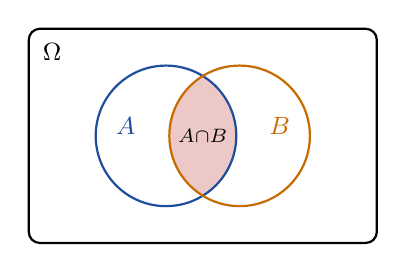
\begin{tikzpicture}[scale=0.85,font=\small]
\draw[thick,rounded corners] (-2.6,-1.6) rectangle (2.6,1.6);
\node at (-2.25,1.25){$\Omega$};
\begin{scope}\clip (-0.55,0) circle (1.05); \fill[cThm!25] (0.55,0) circle (1.05);\end{scope}
\draw[cDef,thick] (-0.55,0) circle (1.05); \draw[cEx,thick] (0.55,0) circle (1.05);
\node[cDef] at (-1.15,0.15){$A$}; \node[cEx] at (1.15,0.15){$B$};
\node[font=\scriptsize] at (0,0){$A{\cap}B$};
\end{tikzpicture}
\end{LTR}\end{center}}

\begin{mithal}
نرمي زهرة نرد ونسجل الرقم الظاهر: $A$: «رقم أكبر تماماً من $3$» ، $B$: «رقم أصغر تماماً من $6$» ، $C$: «رقم زوجي».
\begin{itemize}
\item $\Omega=\{1;2;3;4;5;6\}$ ، \ $A=\{4;5;6\}$ ، \ $B=\{1;2;3;4;5\}$ ، \ $C=\{2;4;6\}$.
\item $A\cap B=\{4;5\}$ ، \ $A\cap C=\{4;6\}$ ، \ $A\cup C=\{2;4;5;6\}$ ، \ $A\cap B\cap C=\{4\}$.
\item $\overline A=\{1;2;3\}$ ، \ $\overline B=\{6\}$ ، \ $\overline{A\cup B}=\overline A\cap\overline B=\varnothing$ ، \ $\overline{A\cap B}=\overline A\cup\overline B=\{1;2;3;6\}$.
\end{itemize}
\end{mithal}

% =====================================================================
\section{قانون الاحتمال على مجموعة منتهية}
\begin{tarif}
$\Omega=\{x_1;x_2;\dots;x_n\}$ مجموعة إمكانيات تجربة عشوائية.\par
نعرّف \textbf{قانون احتمال} $P$ على $\Omega$ بإرفاق كل مخرج $x_i$ بعدد حقيقي $p_i$ (احتماله) بحيث:
\[\bx{0\le p_i\le1}\qquad\text{\ar{و}}\qquad\bx{p_1+p_2+\dots+p_n=1}.\]
نلخص قانون الاحتمال في جدول:
\begin{center}
\renewcommand{\arraystretch}{1.4}
\begin{tabular}{|C|c|c|c|c|c|}\hline
\rowcolor{cSec!12}المخرج $x_i$ & $x_1$ & $x_2$ & $\dots$ & $x_n$ & \ar{المجموع}\\
\hline
الاحتمال $p_i$ & $p_1$ & $p_2$ & $\dots$ & $p_n$ & $1$\\
\hline
\end{tabular}
\end{center}
\end{tarif}

\begin{khassia}[احتمال حادثة]
احتمال حادثة $A$ هو \textbf{مجموع احتمالات المخارج} التي تكوّنها ، ونرمز له بالرمز $P(A)$.\par
$P(\varnothing)=0$ \ ، \ $P(\Omega)=1$ \ ، \ ومن أجل كل حادثة $A$: \ $0\le P(A)\le1$.
\end{khassia}

\begin{mithal}[نرد غير متوازن]
زهرة نرد مزيفة بحيث يكون احتمال ظهور كل رقم فردي ضعف احتمال ظهور كل رقم زوجي.\par
نضع $P(2)=P(4)=P(6)=p$ ، فيكون $P(1)=P(3)=P(5)=2p$.\par
مجموع الاحتمالات يساوي $1$: \ $3\times2p+3\times p=1$ ، أي $9p=1$ ، ومنه $p=\dfrac19$.
\begin{center}
\renewcommand{\arraystretch}{1.5}
\begin{tabular}{|C|c|c|c|c|c|c|c|}\hline
\rowcolor{cSec!12}الرقم & $1$ & $2$ & $3$ & $4$ & $5$ & $6$ & \ar{المجموع}\\
\hline
الاحتمال & $\frac29$ & $\frac19$ & $\frac29$ & $\frac19$ & $\frac29$ & $\frac19$ & $1$\\
\hline
\end{tabular}
\end{center}
احتمال الحادثة $E$: «الحصول على مضاعف للعدد $3$»: \ $E=\{3;6\}$ ، و $P(E)=\dfrac29+\dfrac19=\bx{\dfrac13}$.
\end{mithal}

\begin{molahada}
للتحقق من أن جدولاً يمثل قانون احتمال ، نتحقق من الشرطين: كل الاحتمالات بين $0$ و $1$ ، ومجموعها يساوي $1$.\par
مثلاً: الجدول ذو الاحتمالات $\dfrac34$ ، $-\dfrac14$ ، $\dfrac12$ \textbf{لا} يمثل قانون احتمال (احتمال سالب) ، والجدول ذو الاحتمالات $\dfrac12$ ، $\dfrac14$ ، $\dfrac14$ يمثل قانون احتمال.
\end{molahada}

% =====================================================================
\section{الأمل الرياضياتي والتباين والانحراف المعياري لقانون احتمال}
\begin{tarif}
$\Omega=\{x_1;\dots;x_n\}$ حيث $x_i$ أعداد حقيقية ، و $P$ قانون احتمال على $\Omega$ ($p_i=P(x_i)$).
\begin{itemize}
\item \textbf{الأمل الرياضياتي:} \ \bx{E=\sum_{i=1}^{n}x_ip_i=x_1p_1+x_2p_2+\dots+x_np_n}.
\item \textbf{التباين:} \ \bx{V=\sum_{i=1}^{n}x_i^2p_i-E^2}.
\item \textbf{الانحراف المعياري:} \ \bx{\sigma=\sqrt V}.
\end{itemize}
\end{tarif}
\begin{molahada}
الأمل الرياضياتي هو \textbf{الوسط الحسابي} لقيم $x_i$ إذا اعتبرنا الاحتمالات $p_i$ تواترات نظرية.\par
التباين والانحراف المعياري يقيسان \textbf{تشتت} القيم حول الأمل الرياضياتي.
\end{molahada}
\begin{mithal}
قانون احتمال معرّف على $\Omega=\{-3;2;4;6\}$ بالجدول:
\begin{center}
\renewcommand{\arraystretch}{1.5}
\begin{tabular}{|C|c|c|c|c|}\hline
\rowcolor{cSec!12}$x_i$ & $-3$ & $2$ & $4$ & $6$\\
\hline
$p_i$ & $\frac{2}{12}$ & $\frac{6}{12}$ & $\frac{1}{12}$ & $\frac{3}{12}$\\
\hline
\end{tabular}
\end{center}
\begin{itemize}
\item $E=-3\times\dfrac{2}{12}+2\times\dfrac{6}{12}+4\times\dfrac{1}{12}+6\times\dfrac{3}{12}=\dfrac{-6+12+4+18}{12}=\dfrac{28}{12}=\bx{\dfrac73\approx2{,}33}$.
\item $\displaystyle\sum x_i^2p_i=\dfrac{9\times2+4\times6+16\times1+36\times3}{12}=\dfrac{166}{12}=\dfrac{83}{6}$ ، \quad $V=\dfrac{83}{6}-\Big(\dfrac73\Big)^2=\dfrac{249-98}{18}=\bx{\dfrac{151}{18}\approx8{,}39}$.
\item $\sigma=\sqrt{\dfrac{151}{18}}\approx\bx{2{,}90}$.
\end{itemize}
\end{mithal}

% =====================================================================
\section{تساوي الاحتمال}
\begin{tarif}
نقول إن قانون الاحتمال \textbf{متساوي التوزيع} (أو إن التجربة متساوية الاحتمال) إذا كان لكل المخارج نفس الاحتمال.\par
إذا كان $\card\Omega=n$ فإن احتمال كل مخرج هو $\dfrac1n$.
\end{tarif}
\begin{khassia}
في حالة تساوي الاحتمال ، من أجل كل حادثة $A$:
\[\bx{P(A)=\frac{\card A}{\card\Omega}=\frac{\text{\ar{عدد الحالات الملائمة}}}{\text{\ar{عدد الحالات الممكنة}}}}\]
($\card A$: عدد عناصر $A$.)
\end{khassia}
\begin{molahada}[عبارات تدل على تساوي الاحتمال]
«نرد متوازن» ، «قطعة نقدية متوازنة» ، «كريات متماثلة لا نفرق بينها عند اللمس» ، «نختار عشوائياً» ، «بطاقات متشابهة» $\ldots$\par
\textbf{تنبيه:} في كيس به $3$ كريات حمراء و $4$ خضراء وكرية بيضاء ، إذا سجلنا \textbf{اللون فقط} فإن $\Omega=\{R;V;B\}$ \textbf{ليست} متساوية الاحتمال: $P(R)=\dfrac38$ ، $P(V)=\dfrac48$ ، $P(B)=\dfrac18$. \ لكن إذا رقّمنا الكريات صارت الكريات الثماني متساوية الاحتمال.
\end{molahada}
\begin{mithal}
نرمي نرداً متوازناً. \ $A$: «الحصول على عدد أولي»: $A=\{2;3;5\}$ ، \ $P(A)=\dfrac{3}{6}=\bx{\dfrac12}$.\par
نرمي قطعة نقدية متوازنة مرتين: $\Omega=\{FF;FP;PF;PP\}$. \ $B$: «ظهور الوجه مرة واحدة»: $B=\{FP;PF\}$ ، \ $P(B)=\dfrac24=\bx{\dfrac12}$.
\end{mithal}

% =====================================================================
\section{أدوات العدّ: الجداول المزدوجة وشجرة الإمكانيات}
\begin{khassia}[أنواع السحب من كيس به $n$ كرية (نسحب كريتين)]
\begin{center}
\renewcommand{\arraystretch}{1.6}
\begin{tabular}{|M{0.2\textwidth}|M{0.17\textwidth}|M{0.22\textwidth}|M{0.27\textwidth}|}\hline
\cellcolor{cDef!15}\textbf{الأداة المناسبة} & \cellcolor{cDef!15}\textbf{عدد الحالات} & \cellcolor{cDef!15}\textbf{الترتيب والتكرار} & \cellcolor{cDef!15}\textbf{نوع السحب}\\\hline
جدول مزدوج كامل & $n\times n=n^2$ & الترتيب مهم ، التكرار ممكن & على التوالي \textbf{مع الإرجاع}\\\hline
جدول نشطب قطره & $n(n-1)$ & الترتيب مهم ، لا تكرار & على التوالي \textbf{دون إرجاع}\\\hline
نصف الجدول (فوق القطر) & $\dfrac{n(n-1)}{2}$ & الترتيب غير مهم ، لا تكرار & \textbf{في آن واحد}\\\hline
\end{tabular}
\end{center}
\end{khassia}

\begin{tariqa}[نمذجة تجربة من مرحلتين بجدول مزدوج]
\begin{enumerate}
\item نرقّم العناصر (حتى المتماثلة في اللون) ، فتصبح كل المخارج متساوية الاحتمال.
\item نكتب نتائج المرحلة الأولى في العمود الأول (الأسطر $\text{I}$) ونتائج المرحلة الثانية في السطر الأول (الأعمدة $\text{II}$).
\item كل خانة مخرج واحد. حسب نوع السحب: \textbf{نملأ كل الخانات} (مع الإرجاع) ، أو \textbf{نشطب القطر} (على التوالي دون إرجاع) ، أو \textbf{نملأ ما فوق القطر فقط} (في آن واحد).
\item نلوّن خانات الحادثة $A$ ونعدّها: \quad $P(A)=\dfrac{\text{\ar{عدد الخانات الملونة}}}{\text{\ar{عدد الخانات المملوءة}}}$.
\end{enumerate}
\end{tariqa}

\begin{mithal}[كيس به $3$ كريات بيضاء $B_1$ ، $B_2$ ، $B_3$ وكريتان حمراوان $R_1$ ، $R_2$]
نسحب كريتين ، ونعتبر الحادثة $A$: «سحب كريتين بيضاوين» (الخانات الملونة بالأخضر).

\textbf{1) على التوالي مع الإرجاع:} الكرية الأولى تعود إلى الكيس ، فيمكن سحبها مرة ثانية: \textbf{كل خانات الجدول} مخارج.
\begin{center}\begin{LTR}\renewcommand{\arraystretch}{1.3}
\begin{tabular}{|>{\centering\arraybackslash}m{1.2cm}|>{\centering\arraybackslash}m{1.2cm}|>{\centering\arraybackslash}m{1.2cm}|>{\centering\arraybackslash}m{1.2cm}|>{\centering\arraybackslash}m{1.2cm}|>{\centering\arraybackslash}m{1.2cm}|}\hline
\rowcolor{cSec!12}$\text{I}\backslash\text{II}$ & $B_1$ & $B_2$ & $B_3$ & $R_1$ & $R_2$\\\hline
\cellcolor{cSec!12}$B_1$ & \cellcolor{cRem!25}$B_1B_1$ & \cellcolor{cRem!25}$B_1B_2$ & \cellcolor{cRem!25}$B_1B_3$ & $B_1R_1$ & $B_1R_2$\\\hline
\cellcolor{cSec!12}$B_2$ & \cellcolor{cRem!25}$B_2B_1$ & \cellcolor{cRem!25}$B_2B_2$ & \cellcolor{cRem!25}$B_2B_3$ & $B_2R_1$ & $B_2R_2$\\\hline
\cellcolor{cSec!12}$B_3$ & \cellcolor{cRem!25}$B_3B_1$ & \cellcolor{cRem!25}$B_3B_2$ & \cellcolor{cRem!25}$B_3B_3$ & $B_3R_1$ & $B_3R_2$\\\hline
\cellcolor{cSec!12}$R_1$ & $R_1B_1$ & $R_1B_2$ & $R_1B_3$ & $R_1R_1$ & $R_1R_2$\\\hline
\cellcolor{cSec!12}$R_2$ & $R_2B_1$ & $R_2B_2$ & $R_2B_3$ & $R_2R_1$ & $R_2R_2$\\\hline
\end{tabular}\end{LTR}\end{center}
$\card\Omega=5\times5=25$ \ ، \ $\card A=3\times3=9$ \ ، \ $P(A)=\bx{\dfrac{9}{25}}$.

\textbf{2) على التوالي دون إرجاع:} لا يمكن سحب نفس الكرية مرتين: \textbf{نشطب خانات القطر}.
\begin{center}\begin{LTR}\renewcommand{\arraystretch}{1.3}
\begin{tabular}{|>{\centering\arraybackslash}m{1.2cm}|>{\centering\arraybackslash}m{1.2cm}|>{\centering\arraybackslash}m{1.2cm}|>{\centering\arraybackslash}m{1.2cm}|>{\centering\arraybackslash}m{1.2cm}|>{\centering\arraybackslash}m{1.2cm}|}\hline
\rowcolor{cSec!12}$\text{I}\backslash\text{II}$ & $B_1$ & $B_2$ & $B_3$ & $R_1$ & $R_2$\\\hline
\cellcolor{cSec!12}$B_1$ & \cellcolor{gray!20}$\times$ & \cellcolor{cRem!25}$B_1B_2$ & \cellcolor{cRem!25}$B_1B_3$ & $B_1R_1$ & $B_1R_2$\\\hline
\cellcolor{cSec!12}$B_2$ & \cellcolor{cRem!25}$B_2B_1$ & \cellcolor{gray!20}$\times$ & \cellcolor{cRem!25}$B_2B_3$ & $B_2R_1$ & $B_2R_2$\\\hline
\cellcolor{cSec!12}$B_3$ & \cellcolor{cRem!25}$B_3B_1$ & \cellcolor{cRem!25}$B_3B_2$ & \cellcolor{gray!20}$\times$ & $B_3R_1$ & $B_3R_2$\\\hline
\cellcolor{cSec!12}$R_1$ & $R_1B_1$ & $R_1B_2$ & $R_1B_3$ & \cellcolor{gray!20}$\times$ & $R_1R_2$\\\hline
\cellcolor{cSec!12}$R_2$ & $R_2B_1$ & $R_2B_2$ & $R_2B_3$ & $R_2R_1$ & \cellcolor{gray!20}$\times$\\\hline
\end{tabular}\end{LTR}\end{center}
$\card\Omega=5\times4=20$ \ ، \ $\card A=3\times2=6$ \ ، \ $P(A)=\dfrac{6}{20}=\bx{\dfrac{3}{10}}$.

\textbf{3) في آن واحد:} لا ترتيب: الخانتان $B_1R_1$ و $R_1B_1$ تمثلان نفس السحب $\{B_1;R_1\}$ ، فنحتفظ \textbf{بما فوق القطر فقط}.
\begin{center}\begin{LTR}\renewcommand{\arraystretch}{1.3}
\begin{tabular}{|>{\centering\arraybackslash}m{1.75cm}|>{\centering\arraybackslash}m{1.75cm}|>{\centering\arraybackslash}m{1.75cm}|>{\centering\arraybackslash}m{1.75cm}|>{\centering\arraybackslash}m{1.75cm}|>{\centering\arraybackslash}m{1.75cm}|}\hline
\rowcolor{cSec!12}$\text{I}\backslash\text{II}$ & $B_1$ & $B_2$ & $B_3$ & $R_1$ & $R_2$\\\hline
\cellcolor{cSec!12}$B_1$ & \cellcolor{gray!20} & \cellcolor{cRem!25}$\{B_1;B_2\}$ & \cellcolor{cRem!25}$\{B_1;B_3\}$ & $\{B_1;R_1\}$ & $\{B_1;R_2\}$\\\hline
\cellcolor{cSec!12}$B_2$ & \cellcolor{gray!20} & \cellcolor{gray!20} & \cellcolor{cRem!25}$\{B_2;B_3\}$ & $\{B_2;R_1\}$ & $\{B_2;R_2\}$\\\hline
\cellcolor{cSec!12}$B_3$ & \cellcolor{gray!20} & \cellcolor{gray!20} & \cellcolor{gray!20} & $\{B_3;R_1\}$ & $\{B_3;R_2\}$\\\hline
\cellcolor{cSec!12}$R_1$ & \cellcolor{gray!20} & \cellcolor{gray!20} & \cellcolor{gray!20} & \cellcolor{gray!20} & $\{R_1;R_2\}$\\\hline
\cellcolor{cSec!12}$R_2$ & \cellcolor{gray!20} & \cellcolor{gray!20} & \cellcolor{gray!20} & \cellcolor{gray!20} & \cellcolor{gray!20}\\\hline
\end{tabular}\end{LTR}\end{center}
$\card\Omega=\dfrac{5\times4}{2}=10$ \ ، \ $\card A=\dfrac{3\times2}{2}=3$ \ ، \ $P(A)=\bx{\dfrac{3}{10}}$.
\end{mithal}
\begin{molahada}
السحب في آن واحد والسحب على التوالي دون إرجاع يعطيان نفس الاحتمال ، لأن كل خانة فوق القطر تقابلها خانة واحدة تحته.
\end{molahada}

\begin{mithal}[رمي نرد متوازن مرتين: نكتب في كل خانة مجموع الرقمين]
مع «الإرجاع» (يمكن تكرار الرقم): $6\times6=36$ خانة متساوية الاحتمال. الخانات الملونة: «المجموع يساوي $7$».
\begin{center}\begin{LTR}\renewcommand{\arraystretch}{1.15}
\begin{tabular}{|>{\centering\arraybackslash}m{0.7cm}|>{\centering\arraybackslash}m{0.7cm}|>{\centering\arraybackslash}m{0.7cm}|>{\centering\arraybackslash}m{0.7cm}|>{\centering\arraybackslash}m{0.7cm}|>{\centering\arraybackslash}m{0.7cm}|>{\centering\arraybackslash}m{0.7cm}|}\hline
\rowcolor{cSec!12}$\text{I}\backslash\text{II}$ & $1$ & $2$ & $3$ & $4$ & $5$ & $6$\\\hline
\cellcolor{cSec!12}$1$ & $2$ & $3$ & $4$ & $5$ & $6$ & \cellcolor{cRem!25}$7$\\\hline
\cellcolor{cSec!12}$2$ & $3$ & $4$ & $5$ & $6$ & \cellcolor{cRem!25}$7$ & $8$\\\hline
\cellcolor{cSec!12}$3$ & $4$ & $5$ & $6$ & \cellcolor{cRem!25}$7$ & $8$ & $9$\\\hline
\cellcolor{cSec!12}$4$ & $5$ & $6$ & \cellcolor{cRem!25}$7$ & $8$ & $9$ & $10$\\\hline
\cellcolor{cSec!12}$5$ & $6$ & \cellcolor{cRem!25}$7$ & $8$ & $9$ & $10$ & $11$\\\hline
\cellcolor{cSec!12}$6$ & \cellcolor{cRem!25}$7$ & $8$ & $9$ & $10$ & $11$ & $12$\\\hline
\end{tabular}\end{LTR}\end{center}
$P(\text{\ar{المجموع يساوي}}\ 7)=\dfrac{6}{36}=\bx{\dfrac16}$ \ ؛ \ $P(\text{\ar{نفس الرقم}})=\dfrac{6}{36}=\bx{\dfrac16}$ (خانات القطر).
\end{mithal}

\begin{mithal}[تجربة من ثلاث مراحل: شجرة الإمكانيات]
عندما تتكون التجربة من ثلاث مراحل أو أكثر لا يكفي جدول مزدوج ، فنستعمل \textbf{شجرة الإمكانيات}: كل مسار من الجذر إلى طرف الشجرة مخرج واحد.\par
نرمي قطعة نقدية متوازنة ثلاث مرات:
\begin{center}\begin{LTR}
\begin{tikzpicture}[grow=right,level distance=2.2cm,
 ev/.style={circle,fill=cDef!12,draw=cDef,thick,inner sep=1.5pt,minimum size=0.6cm,font=\small},
 level 1/.style={sibling distance=3.2cm},level 2/.style={sibling distance=1.6cm},level 3/.style={sibling distance=0.8cm},
 edge from parent/.style={draw,cDef!70,thick}]
\node[circle,fill=cDef,inner sep=2pt](r){}
child{node[ev]{$P$}child{node[ev]{$P$}child{node[ev,label={[font=\small]right:{\quad$PPP$}}]{$P$}}child{node[ev,label={[font=\small]right:{\quad$PPF$}}]{$F$}}}child{node[ev]{$F$}child{node[ev,label={[font=\small]right:{\quad$PFP$}}]{$P$}}child{node[ev,label={[font=\small]right:{\quad$PFF$}}]{$F$}}}}child{node[ev]{$F$}child{node[ev]{$P$}child{node[ev,label={[font=\small]right:{\quad$FPP$}}]{$P$}}child{node[ev,label={[font=\small]right:{\quad$FPF$}}]{$F$}}}child{node[ev]{$F$}child{node[ev,label={[font=\small]right:{\quad$FFP$}}]{$P$}}child{node[ev,label={[font=\small]right:{\quad$FFF$}}]{$F$}}}};
\node[font=\bfseries\small,cSec] at (7.6,3.55){\ar{المخرج}};
\foreach \x/\t in {2.2/{الرمية 1},4.4/{الرمية 2},6.6/{الرمية 3}} \node[font=\scriptsize,cSec] at (\x,3.55){\ar{\t}};
\end{tikzpicture}
\end{LTR}\end{center}
عدد المخارج $\card\Omega=2\times2\times2=8$ ، وهي متساوية الاحتمال. \ الحادثة $A$: «ظهور الوجه مرتين بالضبط» تضم المخارج $FFP$ ، $FPF$ ، $PFF$ ، إذن \bx{P(A)=\frac38}.
\end{mithal}

% =====================================================================
\section{خواص الاحتمال}
\begin{khassia}
$P$ قانون احتمال على $\Omega$ ، و $A$ و $B$ حادثتان.
\begin{enumerate}
\item \bx{P(A\cup B)=P(A)+P(B)-P(A\cap B)}.
\item إذا كانت $A$ و $B$ منفصلتين ($A\cap B=\varnothing$): \ \bx{P(A\cup B)=P(A)+P(B)}.
\item \bx{P(\overline A)=1-P(A)} \ (لأن $A$ و $\overline A$ منفصلتان واتحادهما $\Omega$).
\item إذا كان $A\subset B$ فإن $P(A)\le P(B)$.
\end{enumerate}
\end{khassia}
\begin{mithal}
$A$ و $B$ حادثتان حيث: $P(A)=0{,}25$ ، $P(B)=0{,}35$ و $P(A\cap B)=0{,}1$.
\begin{itemize}
\item $P(A\cup B)=0{,}25+0{,}35-0{,}1=\bx{0{,}5}$.
\item $P(\overline A)=1-0{,}25=\bx{0{,}75}$.
\item $P\big(\overline A\cap\overline B\big)=P\big(\overline{A\cup B}\big)=1-0{,}5=\bx{0{,}5}$ \ ؛ \ $P\big(\overline A\cup\overline B\big)=P\big(\overline{A\cap B}\big)=1-0{,}1=\bx{0{,}9}$.
\end{itemize}
\end{mithal}
\begin{tariqa}[متى نستعمل الحادثة العكسية؟]
عندما تحتوي الحادثة على عبارة «\textbf{على الأقل}» نحسب غالباً احتمال عكسها:
\[P(\text{\ar{على الأقل كرية حمراء}})=1-P(\text{\ar{لا توجد أي كرية حمراء}}).\]
\end{tariqa}

% =====================================================================
\section{المتغير العشوائي وقانون احتماله}
\begin{tarif}
$\Omega$ مجموعة إمكانيات تجربة عشوائية. \ نسمي \textbf{متغيراً عشوائياً} $X$ كل دالة ترفق بكل مخرج من $\Omega$ عدداً حقيقياً.\par
مجموعة القيم التي يأخذها $X$ نرمز لها بالرمز $X(\Omega)=\{x_1;x_2;\dots;x_k\}$.\par
$(X=x_i)$ هي الحادثة المكونة من المخارج التي يرفق بها $X$ القيمة $x_i$.
\end{tarif}
\begin{tarif}[قانون احتمال متغير عشوائي]
تعريف قانون احتمال $X$ هو إرفاق كل قيمة $x_i$ باحتمال الحادثة $(X=x_i)$ ، ونلخصه في جدول:
\begin{center}
\renewcommand{\arraystretch}{1.4}
\begin{tabular}{|C|c|c|c|c|c|}\hline
\rowcolor{cSec!12}$x_i$ & $x_1$ & $x_2$ & $\dots$ & $x_k$ & \ar{المجموع}\\
\hline
$P(X=x_i)$ & $p_1$ & $p_2$ & $\dots$ & $p_k$ & $1$\\
\hline
\end{tabular}
\end{center}
\end{tarif}
\begin{tariqa}[طريقة: تعيين قانون احتمال متغير عشوائي]
\begin{enumerate}
\item نعيّن $\Omega$ وعدد عناصرها (جدول أو شجرة).
\item نرفق بكل مخرج قيمة $X$ ، ونستنتج مجموعة القيم $X(\Omega)$.
\item من أجل كل قيمة $x_i$ نعدّ المخارج التي تحقق $(X=x_i)$ ونحسب $P(X=x_i)$.
\item نتحقق أن مجموع الاحتمالات يساوي $1$.
\end{enumerate}
\end{tariqa}

% =====================================================================
\section{الأمل والتباين والانحراف المعياري لمتغير عشوائي}
\begin{tarif}
\begin{itemize}
\item \textbf{الأمل الرياضياتي:} \ \bx{E(X)=\sum_{i=1}^{k}x_i\,P(X=x_i)}.
\item \textbf{التباين:} \ \bx{V(X)=\sum_{i=1}^{k}x_i^2\,P(X=x_i)-\big(E(X)\big)^2}.
\item \textbf{الانحراف المعياري:} \ \bx{\sigma(X)=\sqrt{V(X)}}.
\end{itemize}
\end{tarif}
\begin{molahada}[تفسير الأمل في الألعاب]
إذا كان $X$ يمثل ربح لاعب (موجب) أو خسارته (سالب) ، فإن $E(X)$ هو متوسط الربح الذي يأمله اللاعب بعد تكرار اللعبة عدداً كبيراً من المرات:
\begin{itemize}
\item $E(X)>0$: اللعبة \textbf{في صالح اللاعب} ؛ \quad $E(X)<0$: اللعبة \textbf{ليست في صالحه} ؛ \quad $E(X)=0$: اللعبة \textbf{عادلة}.
\end{itemize}
\end{molahada}
\begin{khassia}[خواص (التحويل التآلفي)]
من أجل كل عددين حقيقيين $a$ و $b$:
\[\bx{E(aX+b)=aE(X)+b}\qquad;\qquad\bx{V(aX+b)=a^2V(X)}\qquad;\qquad\bx{\sigma(aX+b)=|a|\,\sigma(X)}\]
\end{khassia}

\begin{tmr}
يرمي لاعب قطعة نقدية متوازنة ثلاث مرات: يربح دينارا واحدا كلما ظهر الوجه $F$ ويخسر دينارا واحدا كلما ظهر الظهر $P$. \ ليكن $X$ المتغير العشوائي الذي يرفق بكل مخرج ربح اللاعب أو خسارته.
\begin{enumerate}
\item عيّن قيم $X$ وقانون احتماله.
\item احسب $E(X)$ ، $V(X)$ و $\sigma(X)$. \ هل اللعبة عادلة؟
\item استنتج $E(2X+3)$ و $\sigma(-3X+1)$.
\end{enumerate}
\end{tmr}
\begin{hal}
\textbf{1.} $\card\Omega=8$ (الشجرة السابقة). \ إذا ظهر الوجه $k$ مرة والظهر $3-k$ مرة فإن $X=k-(3-k)=2k-3$:
\begin{itemize}
\item $FFF\to3$ \ ؛ \ $FFP$ ، $FPF$ ، $PFF\to1$ \ ؛ \ $FPP$ ، $PFP$ ، $PPF\to-1$ \ ؛ \ $PPP\to-3$.
\end{itemize}
$X(\Omega)=\{-3;-1;1;3\}$:
\begin{center}
\renewcommand{\arraystretch}{1.5}
\begin{tabular}{|C|c|c|c|c|c|}\hline
\rowcolor{cSec!12}$x_i$ & $-3$ & $-1$ & $1$ & $3$ & \ar{المجموع}\\
\hline
$P(X=x_i)$ & $\frac18$ & $\frac38$ & $\frac38$ & $\frac18$ & $1$\\
\hline
\end{tabular}
\end{center}
\textbf{2.} $E(X)=\dfrac{-3-3+3+3}{8}=\bx{0}$: اللعبة \textbf{عادلة}.\par
$V(X)=\dfrac{9\times1+1\times3+1\times3+9\times1}{8}-0^2=\dfrac{24}{8}=\bx{3}$ ، \quad $\sigma(X)=\bx{\sqrt3\approx1{,}73}$.\par
\textbf{3.} $E(2X+3)=2E(X)+3=\bx{3}$ \ ؛ \ $\sigma(-3X+1)=|-3|\,\sigma(X)=\bx{3\sqrt3}$.
\end{hal}

% =====================================================================
\section{خلاصة الطرائق}
\begin{BOX}{cMeth}{ماذا أفعل عندما يُطلب مني $\ldots$؟}
\renewcommand{\arraystretch}{1.5}
\centering
\begin{tabular}{|p{0.5\textwidth}|p{0.38\textwidth}|}\hline
\cellcolor{cMeth!15}\textbf{الطريقة} & \cellcolor{cMeth!15}\textbf{المطلوب}\\\hline
شجرة (عدة مراحل) أو جدول مزدوج (مرحلتان) حسب نوع السحب. & تعيين $\Omega$ وعدد الحالات\\\hline
$P(A)=\dfrac{\card A}{\card\Omega}$ (بعد التأكد من تساوي الاحتمال). & احتمال حادثة في تجربة متساوية الاحتمال\\\hline
مجموع احتمالات مخارجها. & احتمال حادثة في قانون غير متساوي التوزيع\\\hline
$1-P(\text{\ar{العكسية}})$. & احتمال «على الأقل $\ldots$»\\\hline
$P(A)+P(B)-P(A\cap B)$. & احتمال «$A$ أو $B$»\\\hline
نستعمل: مجموع الاحتمالات $=1$ ، أو قيمة معطاة للأمل. & إيجاد احتمال مجهول في جدول\\\hline
$\sum x_ip_i$ ، ثم $\sum x_i^2p_i-E^2$ ، ثم الجذر. & الأمل ، التباين ، الانحراف المعياري\\\hline
إشارة $E(X)$: موجب (في صالحه) ، معدوم (عادلة). & هل اللعبة في صالح اللاعب؟\\\hline
\end{tabular}
\end{BOX}

\end{document}
